\documentclass[twoside]{book}

% Packages required by doxygen
\usepackage{fixltx2e}
\usepackage{calc}
\usepackage{doxygen}
\usepackage[export]{adjustbox} % also loads graphicx
\usepackage{graphicx}
\usepackage[utf8]{inputenc}
\usepackage{makeidx}
\usepackage{multicol}
\usepackage{multirow}
\PassOptionsToPackage{warn}{textcomp}
\usepackage{textcomp}
\usepackage[nointegrals]{wasysym}
\usepackage[table]{xcolor}

% Font selection
\usepackage[T1]{fontenc}
\usepackage[scaled=.90]{helvet}
\usepackage{courier}
\usepackage{amssymb}
\usepackage{sectsty}
\renewcommand{\familydefault}{\sfdefault}
\allsectionsfont{%
  \fontseries{bc}\selectfont%
  \color{darkgray}%
}
\renewcommand{\DoxyLabelFont}{%
  \fontseries{bc}\selectfont%
  \color{darkgray}%
}
\newcommand{\+}{\discretionary{\mbox{\scriptsize$\hookleftarrow$}}{}{}}

% Page & text layout
\usepackage{geometry}
\geometry{%
  a4paper,%
  top=2.5cm,%
  bottom=2.5cm,%
  left=2.5cm,%
  right=2.5cm%
}
\tolerance=750
\hfuzz=15pt
\hbadness=750
\setlength{\emergencystretch}{15pt}
\setlength{\parindent}{0cm}
\setlength{\parskip}{3ex plus 2ex minus 2ex}
\makeatletter
\renewcommand{\paragraph}{%
  \@startsection{paragraph}{4}{0ex}{-1.0ex}{1.0ex}{%
    \normalfont\normalsize\bfseries\SS@parafont%
  }%
}
\renewcommand{\subparagraph}{%
  \@startsection{subparagraph}{5}{0ex}{-1.0ex}{1.0ex}{%
    \normalfont\normalsize\bfseries\SS@subparafont%
  }%
}
\makeatother

% Headers & footers
\usepackage{fancyhdr}
\pagestyle{fancyplain}
\fancyhead[LE]{\fancyplain{}{\bfseries\thepage}}
\fancyhead[CE]{\fancyplain{}{}}
\fancyhead[RE]{\fancyplain{}{\bfseries\leftmark}}
\fancyhead[LO]{\fancyplain{}{\bfseries\rightmark}}
\fancyhead[CO]{\fancyplain{}{}}
\fancyhead[RO]{\fancyplain{}{\bfseries\thepage}}
\fancyfoot[LE]{\fancyplain{}{}}
\fancyfoot[CE]{\fancyplain{}{}}
\fancyfoot[RE]{\fancyplain{}{\bfseries\scriptsize Generated by Doxygen }}
\fancyfoot[LO]{\fancyplain{}{\bfseries\scriptsize Generated by Doxygen }}
\fancyfoot[CO]{\fancyplain{}{}}
\fancyfoot[RO]{\fancyplain{}{}}
\renewcommand{\footrulewidth}{0.4pt}
\renewcommand{\chaptermark}[1]{%
  \markboth{#1}{}%
}
\renewcommand{\sectionmark}[1]{%
  \markright{\thesection\ #1}%
}

% Indices & bibliography
\usepackage{natbib}
\usepackage[titles]{tocloft}
\setcounter{tocdepth}{3}
\setcounter{secnumdepth}{5}
\makeindex

% Hyperlinks (required, but should be loaded last)
\usepackage{ifpdf}
\ifpdf
  \usepackage[pdftex,pagebackref=true]{hyperref}
\else
  \usepackage[ps2pdf,pagebackref=true]{hyperref}
\fi
\hypersetup{%
  colorlinks=true,%
  linkcolor=blue,%
  citecolor=blue,%
  unicode%
}

% Custom commands
\newcommand{\clearemptydoublepage}{%
  \newpage{\pagestyle{empty}\cleardoublepage}%
}

\usepackage{caption}
\captionsetup{labelsep=space,justification=centering,font={bf},singlelinecheck=off,skip=4pt,position=top}

%===== C O N T E N T S =====

\begin{document}

% Titlepage & ToC
\hypersetup{pageanchor=false,
             bookmarksnumbered=true,
             pdfencoding=unicode
            }
\pagenumbering{alph}
\begin{titlepage}
\vspace*{7cm}
\begin{center}%
{\Large Mike\+Simulator }\\
\vspace*{1cm}
{\large Generated by Doxygen 1.8.13}\\
\end{center}
\end{titlepage}
\clearemptydoublepage
\pagenumbering{roman}
\tableofcontents
\clearemptydoublepage
\pagenumbering{arabic}
\hypersetup{pageanchor=true}

%--- Begin generated contents ---
\chapter{Main Page}
\label{index}\hypertarget{index}{}Description of this software\+:

A simulator to train how to trade live markets using custom designed algos; using live data but also \textquotesingle{}manual data\textquotesingle{} to understand what happens to algo orders when price moves. Manual data means bid/ask prices controlled by the user -\/ to simulate market moves I want to analyse. There will be a lot of different algos to develop and try out. Some fully autonomous, most launched by user and used as \textquotesingle{}bots\textquotesingle{}

Features\+:

Connect to Interactive brokers

Pull live market data from Interactive Brokers

Use that data for trading

be able to\+:

save that live market data to file

use that saved data as historic data for future simulations

be able to switch off live data and go to \textquotesingle{}hand control\textquotesingle{} where I decide what the price does manually to check behaviour of algos

initially, fills are handled locally -\/ all longs fill at ask and shorts at bid. at some point, this will be changed so that fills are handled by Interactive Brokers and this software only checks if an order was filled or not.

design considerations\+:

Make it easy to grow and add new feautres.

enable adding new algos at later stage.

enable adding new ways to display current positions later.

enagle adding new G\+UI to deal with postitions, orders and algos.

enable adding new features to \textquotesingle{}Data\textquotesingle{} class -\/ trading multiple different instruments instead of just one, saving live price streams to file, loading those streams from file -\/ to use historical data instead of live data, \textquotesingle{}speeding up\textquotesingle{}, stopping and starting the flow of historical bid/ask prices to analyse algo behaviour using past historical data 
\chapter{Namespace Index}
\section{Namespace List}
Here is a list of all namespaces with brief descriptions\+:\begin{DoxyCompactList}
\item\contentsline{section}{\hyperlink{namespace_mike}{Mike} }{\pageref{namespace_mike}}{}
\end{DoxyCompactList}

\chapter{Class Index}
\section{Class List}
Here are the classes, structs, unions and interfaces with brief descriptions\+:\begin{DoxyCompactList}
\item\contentsline{section}{\hyperlink{class_mike_1_1_control}{Mike\+::\+Control} }{\pageref{class_mike_1_1_control}}{}
\item\contentsline{section}{\hyperlink{class_control_u_i}{Control\+UI} }{\pageref{class_control_u_i}}{}
\item\contentsline{section}{\hyperlink{class_mike_1_1_data}{Mike\+::\+Data} }{\pageref{class_mike_1_1_data}}{}
\item\contentsline{section}{\hyperlink{class_fluid_control_interface}{Fluid\+Control\+Interface} }{\pageref{class_fluid_control_interface}}{}
\item\contentsline{section}{\hyperlink{class_fluid_interface}{Fluid\+Interface} }{\pageref{class_fluid_interface}}{}
\item\contentsline{section}{\hyperlink{class_fluid_price_control_u_i}{Fluid\+Price\+Control\+UI} }{\pageref{class_fluid_price_control_u_i}}{}
\item\contentsline{section}{\hyperlink{class_mike_1_1_mike_order}{Mike\+::\+Mike\+Order} }{\pageref{class_mike_1_1_mike_order}}{}
\item\contentsline{section}{\hyperlink{class_mike_1_1_mike_orders_at_price}{Mike\+::\+Mike\+Orders\+At\+Price} }{\pageref{class_mike_1_1_mike_orders_at_price}}{}
\item\contentsline{section}{\hyperlink{class_mike_1_1_mike_position}{Mike\+::\+Mike\+Position} }{\pageref{class_mike_1_1_mike_position}}{}
\item\contentsline{section}{\hyperlink{class_mike_u_i}{Mike\+UI} }{\pageref{class_mike_u_i}}{}
\item\contentsline{section}{\hyperlink{class_mike_1_1_my__fl__button}{Mike\+::\+My\+\_\+fl\+\_\+button} }{\pageref{class_mike_1_1_my__fl__button}}{}
\item\contentsline{section}{\hyperlink{class_mike_1_1_user_interface}{Mike\+::\+User\+Interface} }{\pageref{class_mike_1_1_user_interface}}{}
\item\contentsline{section}{\hyperlink{class_mike_1_1_user_interface_base}{Mike\+::\+User\+Interface\+Base} }{\pageref{class_mike_1_1_user_interface_base}}{}
\item\contentsline{section}{\hyperlink{class_mike_1_1_user_interface_linked}{Mike\+::\+User\+Interface\+Linked} }{\pageref{class_mike_1_1_user_interface_linked}}{}
\item\contentsline{section}{\hyperlink{class_mike_1_1_widget_table}{Mike\+::\+Widget\+Table} }{\pageref{class_mike_1_1_widget_table}}{}
\item\contentsline{section}{\hyperlink{class_mike_1_1_wid_table_base}{Mike\+::\+Wid\+Table\+Base} }{\pageref{class_mike_1_1_wid_table_base}}{}
\end{DoxyCompactList}

\chapter{File Index}
\section{File List}
Here is a list of all files with brief descriptions\+:\begin{DoxyCompactList}
\item\contentsline{section}{F\+L\+U\+I\+D/\hyperlink{_fluid_control_interface_8cxx}{Fluid\+Control\+Interface.\+cxx} }{\pageref{_fluid_control_interface_8cxx}}{}
\item\contentsline{section}{F\+L\+U\+I\+D/\hyperlink{_fluid_control_interface_8h}{Fluid\+Control\+Interface.\+h} }{\pageref{_fluid_control_interface_8h}}{}
\item\contentsline{section}{F\+L\+U\+I\+D/\hyperlink{_fluid_price_control_8cxx}{Fluid\+Price\+Control.\+cxx} }{\pageref{_fluid_price_control_8cxx}}{}
\item\contentsline{section}{F\+L\+U\+I\+D/\hyperlink{_fluid_price_control_8h}{Fluid\+Price\+Control.\+h} }{\pageref{_fluid_price_control_8h}}{}
\item\contentsline{section}{src/\hyperlink{_control_8cpp}{Control.\+cpp} }{\pageref{_control_8cpp}}{}
\item\contentsline{section}{src/\hyperlink{_control_8h}{Control.\+h} }{\pageref{_control_8h}}{}
\item\contentsline{section}{src/\hyperlink{main_8cpp}{main.\+cpp} }{\pageref{main_8cpp}}{}
\item\contentsline{section}{src/\hyperlink{_mike_enums_8h}{Mike\+Enums.\+h} }{\pageref{_mike_enums_8h}}{}
\end{DoxyCompactList}

\chapter{Namespace Documentation}
\hypertarget{namespace_mike}{}\section{Mike Namespace Reference}
\label{namespace_mike}\index{Mike@{Mike}}
\subsection*{Classes}
\begin{DoxyCompactItemize}
\item 
class \hyperlink{class_mike_1_1_control}{Control}
\item 
class \hyperlink{class_mike_1_1_data}{Data}
\item 
class \hyperlink{class_mike_1_1_mike_order}{Mike\+Order}
\item 
class \hyperlink{class_mike_1_1_mike_orders_at_price}{Mike\+Orders\+At\+Price}
\item 
class \hyperlink{class_mike_1_1_mike_position}{Mike\+Position}
\item 
class \hyperlink{class_mike_1_1_my__fl__button}{My\+\_\+fl\+\_\+button}
\item 
class \hyperlink{class_mike_1_1_user_interface}{User\+Interface}
\item 
class \hyperlink{class_mike_1_1_user_interface_base}{User\+Interface\+Base}
\item 
class \hyperlink{class_mike_1_1_user_interface_linked}{User\+Interface\+Linked}
\item 
class \hyperlink{class_mike_1_1_widget_table}{Widget\+Table}
\item 
class \hyperlink{class_mike_1_1_wid_table_base}{Wid\+Table\+Base}
\end{DoxyCompactItemize}
\subsection*{Enumerations}
\begin{DoxyCompactItemize}
\item 
enum \hyperlink{namespace_mike_aa486aea8b1d0d07190982a311394e6cb}{Mike\+Order\+Type} \{ \newline
\hyperlink{namespace_mike_aa486aea8b1d0d07190982a311394e6cba80f009cd3767a52807d46f46317b2010}{C\+X\+L\+O\+R\+D\+ER}, 
\hyperlink{namespace_mike_aa486aea8b1d0d07190982a311394e6cba95eacef5178d46e4cacf51432bd802d1}{B\+U\+Y\+L\+MT}, 
\hyperlink{namespace_mike_aa486aea8b1d0d07190982a311394e6cba790d25ece8bd5d94f9eb23a4d1495e01}{B\+U\+Y\+S\+TP}, 
\hyperlink{namespace_mike_aa486aea8b1d0d07190982a311394e6cbaf25ad558ba1e65b2855cbbe63d73c33b}{S\+E\+L\+L\+L\+MT}, 
\newline
\hyperlink{namespace_mike_aa486aea8b1d0d07190982a311394e6cbafa61ee0a04fd985863c9b3015beab7e3}{S\+E\+L\+L\+S\+TP}
 \}
\item 
enum \hyperlink{namespace_mike_a9dd611fa3c671b02e477e6b21465cc66}{Btn\+Pressed} \{ \newline
\hyperlink{namespace_mike_a9dd611fa3c671b02e477e6b21465cc66afe84ab8fffe0adb5a7f80f7fc92b3eac}{Btn\+Pressed\+::\+U\+P\+B\+TN}, 
\hyperlink{namespace_mike_a9dd611fa3c671b02e477e6b21465cc66a46d3bb51d595458598fa22b21480e5cb}{Btn\+Pressed\+::\+D\+O\+W\+N\+B\+TN}, 
\hyperlink{namespace_mike_a9dd611fa3c671b02e477e6b21465cc66a2f29ae51ab6f869980ca89cd5f2ee9e0}{Btn\+Pressed\+::\+E\+X\+T\+R\+A\+B\+TN}, 
\hyperlink{namespace_mike_a9dd611fa3c671b02e477e6b21465cc66ac1d632c96d763edcce1ebba77b0ba5a4}{Btn\+Pressed\+::\+S\+L\+I\+D\+E\+R1}, 
\newline
\hyperlink{namespace_mike_a9dd611fa3c671b02e477e6b21465cc66ad88061c53bebad3a332240e1ae155360}{Btn\+Pressed\+::\+N\+E\+X\+T\+B\+TN}, 
\hyperlink{namespace_mike_a9dd611fa3c671b02e477e6b21465cc66a790d81bf8b9805f17946ec3bac50f1c5}{Btn\+Pressed\+::\+P\+R\+E\+V\+B\+TN}, 
\hyperlink{namespace_mike_a9dd611fa3c671b02e477e6b21465cc66a69e18a8cb5f22f0d83283af4fb3c356c}{Btn\+Pressed\+::\+P\+R\+I\+N\+T\+O\+R\+D\+E\+R\+S\+B\+TN}, 
\hyperlink{namespace_mike_a9dd611fa3c671b02e477e6b21465cc66ac3c5f946beebdf7f30a2d06348be59a4}{Btn\+Pressed\+::\+C\+H\+E\+C\+K\+F\+I\+L\+LS}, 
\newline
\hyperlink{namespace_mike_a9dd611fa3c671b02e477e6b21465cc66ada98a68cf3852968ae256b4dcb2bcad1}{Btn\+Pressed\+::\+P\+R\+I\+N\+T\+P\+OS}, 
\hyperlink{namespace_mike_a9dd611fa3c671b02e477e6b21465cc66ad2415eb73ce7a66a15aa59d80509b203}{Btn\+Pressed\+::\+P\+R\+I\+N\+T\+B\+UT}, 
\hyperlink{namespace_mike_a9dd611fa3c671b02e477e6b21465cc66a8602647ca2d135532c33ebf597ec1199}{Btn\+Pressed\+::\+L\+I\+V\+E\+D\+A\+T\+A\+C\+O\+N\+S\+O\+L\+E\+P\+R\+I\+N\+T\+O\+UT}, 
\hyperlink{namespace_mike_a9dd611fa3c671b02e477e6b21465cc66a66d7f181c31512aa2aa39a7bfac160cc}{Btn\+Pressed\+::\+C\+O\+N\+N\+E\+C\+T\+L\+I\+V\+E\+D\+A\+TA}, 
\newline
\hyperlink{namespace_mike_a9dd611fa3c671b02e477e6b21465cc66afdd7056a8336913761e5b22e5094b13f}{Btn\+Pressed\+::\+S\+T\+A\+R\+T\+L\+O\+OP}, 
\hyperlink{namespace_mike_a9dd611fa3c671b02e477e6b21465cc66a8df329b49b6668b7b1ec13ba71c72864}{Btn\+Pressed\+::\+E\+X\+P\+E\+R\+I\+M\+E\+NT}, 
\hyperlink{namespace_mike_a9dd611fa3c671b02e477e6b21465cc66ad80f2da521c72deea940b13dc9c55138}{Btn\+Pressed\+::\+C\+A\+N\+C\+E\+L\+A\+L\+L\+O\+R\+D\+E\+RS}, 
\hyperlink{namespace_mike_a9dd611fa3c671b02e477e6b21465cc66ab26db120255197418962e537e3e5e301}{Btn\+Pressed\+::\+C\+L\+E\+A\+R\+A\+L\+L\+P\+O\+S\+I\+T\+I\+O\+NS}
 \}
\item 
enum \hyperlink{namespace_mike_a194f722ae64bec13b06019160da629c6}{Order\+Status} \{ \hyperlink{namespace_mike_a194f722ae64bec13b06019160da629c6aa38bd5138bf35514df41a1795ebbf5c3}{Order\+Status\+::\+O\+P\+EN}, 
\hyperlink{namespace_mike_a194f722ae64bec13b06019160da629c6a5b053ae8b6dc09eed2aa8c3a07163a7a}{Order\+Status\+::\+F\+I\+L\+L\+ED}, 
\hyperlink{namespace_mike_a194f722ae64bec13b06019160da629c6a2eed1f37802fbc2235e1a112aebb49d9}{Order\+Status\+::\+P\+A\+R\+T\+F\+I\+LL}, 
\hyperlink{namespace_mike_a194f722ae64bec13b06019160da629c6a9f935beb31030ad0d4d26126c0f39bf2}{Order\+Status\+::\+C\+A\+N\+C\+E\+L\+L\+ED}
 \}
\end{DoxyCompactItemize}
\subsection*{Functions}
\begin{DoxyCompactItemize}
\item 
int \hyperlink{namespace_mike_ada7afe897748f668730c74456952e356}{frequency\+\_\+of\+\_\+primes} (int n)
\end{DoxyCompactItemize}
\subsection*{Variables}
\begin{DoxyCompactItemize}
\item 
static const double \hyperlink{namespace_mike_abbeda217f93388b7dd036c32d183f426}{S\+E\+T\+\_\+\+M\+A\+I\+N\+L\+O\+O\+P\+\_\+\+I\+N\+T\+E\+R\+V\+AL} = 0.\+01
\end{DoxyCompactItemize}


\subsection{Enumeration Type Documentation}
\mbox{\Hypertarget{namespace_mike_a9dd611fa3c671b02e477e6b21465cc66}\label{namespace_mike_a9dd611fa3c671b02e477e6b21465cc66}} 
\index{Mike@{Mike}!Btn\+Pressed@{Btn\+Pressed}}
\index{Btn\+Pressed@{Btn\+Pressed}!Mike@{Mike}}
\subsubsection{\texorpdfstring{Btn\+Pressed}{BtnPressed}}
{\footnotesize\ttfamily enum \hyperlink{namespace_mike_a9dd611fa3c671b02e477e6b21465cc66}{Mike\+::\+Btn\+Pressed}\hspace{0.3cm}{\ttfamily [strong]}}

\begin{DoxyEnumFields}{Enumerator}
\raisebox{\heightof{T}}[0pt][0pt]{\index{U\+P\+B\+TN@{U\+P\+B\+TN}!Mike@{Mike}}\index{Mike@{Mike}!U\+P\+B\+TN@{U\+P\+B\+TN}}}\mbox{\Hypertarget{namespace_mike_a9dd611fa3c671b02e477e6b21465cc66afe84ab8fffe0adb5a7f80f7fc92b3eac}\label{namespace_mike_a9dd611fa3c671b02e477e6b21465cc66afe84ab8fffe0adb5a7f80f7fc92b3eac}} 
U\+P\+B\+TN&\\
\hline

\raisebox{\heightof{T}}[0pt][0pt]{\index{D\+O\+W\+N\+B\+TN@{D\+O\+W\+N\+B\+TN}!Mike@{Mike}}\index{Mike@{Mike}!D\+O\+W\+N\+B\+TN@{D\+O\+W\+N\+B\+TN}}}\mbox{\Hypertarget{namespace_mike_a9dd611fa3c671b02e477e6b21465cc66a46d3bb51d595458598fa22b21480e5cb}\label{namespace_mike_a9dd611fa3c671b02e477e6b21465cc66a46d3bb51d595458598fa22b21480e5cb}} 
D\+O\+W\+N\+B\+TN&\\
\hline

\raisebox{\heightof{T}}[0pt][0pt]{\index{E\+X\+T\+R\+A\+B\+TN@{E\+X\+T\+R\+A\+B\+TN}!Mike@{Mike}}\index{Mike@{Mike}!E\+X\+T\+R\+A\+B\+TN@{E\+X\+T\+R\+A\+B\+TN}}}\mbox{\Hypertarget{namespace_mike_a9dd611fa3c671b02e477e6b21465cc66a2f29ae51ab6f869980ca89cd5f2ee9e0}\label{namespace_mike_a9dd611fa3c671b02e477e6b21465cc66a2f29ae51ab6f869980ca89cd5f2ee9e0}} 
E\+X\+T\+R\+A\+B\+TN&\\
\hline

\raisebox{\heightof{T}}[0pt][0pt]{\index{S\+L\+I\+D\+E\+R1@{S\+L\+I\+D\+E\+R1}!Mike@{Mike}}\index{Mike@{Mike}!S\+L\+I\+D\+E\+R1@{S\+L\+I\+D\+E\+R1}}}\mbox{\Hypertarget{namespace_mike_a9dd611fa3c671b02e477e6b21465cc66ac1d632c96d763edcce1ebba77b0ba5a4}\label{namespace_mike_a9dd611fa3c671b02e477e6b21465cc66ac1d632c96d763edcce1ebba77b0ba5a4}} 
S\+L\+I\+D\+E\+R1&\\
\hline

\raisebox{\heightof{T}}[0pt][0pt]{\index{N\+E\+X\+T\+B\+TN@{N\+E\+X\+T\+B\+TN}!Mike@{Mike}}\index{Mike@{Mike}!N\+E\+X\+T\+B\+TN@{N\+E\+X\+T\+B\+TN}}}\mbox{\Hypertarget{namespace_mike_a9dd611fa3c671b02e477e6b21465cc66ad88061c53bebad3a332240e1ae155360}\label{namespace_mike_a9dd611fa3c671b02e477e6b21465cc66ad88061c53bebad3a332240e1ae155360}} 
N\+E\+X\+T\+B\+TN&\\
\hline

\raisebox{\heightof{T}}[0pt][0pt]{\index{P\+R\+E\+V\+B\+TN@{P\+R\+E\+V\+B\+TN}!Mike@{Mike}}\index{Mike@{Mike}!P\+R\+E\+V\+B\+TN@{P\+R\+E\+V\+B\+TN}}}\mbox{\Hypertarget{namespace_mike_a9dd611fa3c671b02e477e6b21465cc66a790d81bf8b9805f17946ec3bac50f1c5}\label{namespace_mike_a9dd611fa3c671b02e477e6b21465cc66a790d81bf8b9805f17946ec3bac50f1c5}} 
P\+R\+E\+V\+B\+TN&\\
\hline

\raisebox{\heightof{T}}[0pt][0pt]{\index{P\+R\+I\+N\+T\+O\+R\+D\+E\+R\+S\+B\+TN@{P\+R\+I\+N\+T\+O\+R\+D\+E\+R\+S\+B\+TN}!Mike@{Mike}}\index{Mike@{Mike}!P\+R\+I\+N\+T\+O\+R\+D\+E\+R\+S\+B\+TN@{P\+R\+I\+N\+T\+O\+R\+D\+E\+R\+S\+B\+TN}}}\mbox{\Hypertarget{namespace_mike_a9dd611fa3c671b02e477e6b21465cc66a69e18a8cb5f22f0d83283af4fb3c356c}\label{namespace_mike_a9dd611fa3c671b02e477e6b21465cc66a69e18a8cb5f22f0d83283af4fb3c356c}} 
P\+R\+I\+N\+T\+O\+R\+D\+E\+R\+S\+B\+TN&\\
\hline

\raisebox{\heightof{T}}[0pt][0pt]{\index{C\+H\+E\+C\+K\+F\+I\+L\+LS@{C\+H\+E\+C\+K\+F\+I\+L\+LS}!Mike@{Mike}}\index{Mike@{Mike}!C\+H\+E\+C\+K\+F\+I\+L\+LS@{C\+H\+E\+C\+K\+F\+I\+L\+LS}}}\mbox{\Hypertarget{namespace_mike_a9dd611fa3c671b02e477e6b21465cc66ac3c5f946beebdf7f30a2d06348be59a4}\label{namespace_mike_a9dd611fa3c671b02e477e6b21465cc66ac3c5f946beebdf7f30a2d06348be59a4}} 
C\+H\+E\+C\+K\+F\+I\+L\+LS&\\
\hline

\raisebox{\heightof{T}}[0pt][0pt]{\index{P\+R\+I\+N\+T\+P\+OS@{P\+R\+I\+N\+T\+P\+OS}!Mike@{Mike}}\index{Mike@{Mike}!P\+R\+I\+N\+T\+P\+OS@{P\+R\+I\+N\+T\+P\+OS}}}\mbox{\Hypertarget{namespace_mike_a9dd611fa3c671b02e477e6b21465cc66ada98a68cf3852968ae256b4dcb2bcad1}\label{namespace_mike_a9dd611fa3c671b02e477e6b21465cc66ada98a68cf3852968ae256b4dcb2bcad1}} 
P\+R\+I\+N\+T\+P\+OS&\\
\hline

\raisebox{\heightof{T}}[0pt][0pt]{\index{P\+R\+I\+N\+T\+B\+UT@{P\+R\+I\+N\+T\+B\+UT}!Mike@{Mike}}\index{Mike@{Mike}!P\+R\+I\+N\+T\+B\+UT@{P\+R\+I\+N\+T\+B\+UT}}}\mbox{\Hypertarget{namespace_mike_a9dd611fa3c671b02e477e6b21465cc66ad2415eb73ce7a66a15aa59d80509b203}\label{namespace_mike_a9dd611fa3c671b02e477e6b21465cc66ad2415eb73ce7a66a15aa59d80509b203}} 
P\+R\+I\+N\+T\+B\+UT&\\
\hline

\raisebox{\heightof{T}}[0pt][0pt]{\index{L\+I\+V\+E\+D\+A\+T\+A\+C\+O\+N\+S\+O\+L\+E\+P\+R\+I\+N\+T\+O\+UT@{L\+I\+V\+E\+D\+A\+T\+A\+C\+O\+N\+S\+O\+L\+E\+P\+R\+I\+N\+T\+O\+UT}!Mike@{Mike}}\index{Mike@{Mike}!L\+I\+V\+E\+D\+A\+T\+A\+C\+O\+N\+S\+O\+L\+E\+P\+R\+I\+N\+T\+O\+UT@{L\+I\+V\+E\+D\+A\+T\+A\+C\+O\+N\+S\+O\+L\+E\+P\+R\+I\+N\+T\+O\+UT}}}\mbox{\Hypertarget{namespace_mike_a9dd611fa3c671b02e477e6b21465cc66a8602647ca2d135532c33ebf597ec1199}\label{namespace_mike_a9dd611fa3c671b02e477e6b21465cc66a8602647ca2d135532c33ebf597ec1199}} 
L\+I\+V\+E\+D\+A\+T\+A\+C\+O\+N\+S\+O\+L\+E\+P\+R\+I\+N\+T\+O\+UT&\\
\hline

\raisebox{\heightof{T}}[0pt][0pt]{\index{C\+O\+N\+N\+E\+C\+T\+L\+I\+V\+E\+D\+A\+TA@{C\+O\+N\+N\+E\+C\+T\+L\+I\+V\+E\+D\+A\+TA}!Mike@{Mike}}\index{Mike@{Mike}!C\+O\+N\+N\+E\+C\+T\+L\+I\+V\+E\+D\+A\+TA@{C\+O\+N\+N\+E\+C\+T\+L\+I\+V\+E\+D\+A\+TA}}}\mbox{\Hypertarget{namespace_mike_a9dd611fa3c671b02e477e6b21465cc66a66d7f181c31512aa2aa39a7bfac160cc}\label{namespace_mike_a9dd611fa3c671b02e477e6b21465cc66a66d7f181c31512aa2aa39a7bfac160cc}} 
C\+O\+N\+N\+E\+C\+T\+L\+I\+V\+E\+D\+A\+TA&\\
\hline

\raisebox{\heightof{T}}[0pt][0pt]{\index{S\+T\+A\+R\+T\+L\+O\+OP@{S\+T\+A\+R\+T\+L\+O\+OP}!Mike@{Mike}}\index{Mike@{Mike}!S\+T\+A\+R\+T\+L\+O\+OP@{S\+T\+A\+R\+T\+L\+O\+OP}}}\mbox{\Hypertarget{namespace_mike_a9dd611fa3c671b02e477e6b21465cc66afdd7056a8336913761e5b22e5094b13f}\label{namespace_mike_a9dd611fa3c671b02e477e6b21465cc66afdd7056a8336913761e5b22e5094b13f}} 
S\+T\+A\+R\+T\+L\+O\+OP&\\
\hline

\raisebox{\heightof{T}}[0pt][0pt]{\index{E\+X\+P\+E\+R\+I\+M\+E\+NT@{E\+X\+P\+E\+R\+I\+M\+E\+NT}!Mike@{Mike}}\index{Mike@{Mike}!E\+X\+P\+E\+R\+I\+M\+E\+NT@{E\+X\+P\+E\+R\+I\+M\+E\+NT}}}\mbox{\Hypertarget{namespace_mike_a9dd611fa3c671b02e477e6b21465cc66a8df329b49b6668b7b1ec13ba71c72864}\label{namespace_mike_a9dd611fa3c671b02e477e6b21465cc66a8df329b49b6668b7b1ec13ba71c72864}} 
E\+X\+P\+E\+R\+I\+M\+E\+NT&\\
\hline

\raisebox{\heightof{T}}[0pt][0pt]{\index{C\+A\+N\+C\+E\+L\+A\+L\+L\+O\+R\+D\+E\+RS@{C\+A\+N\+C\+E\+L\+A\+L\+L\+O\+R\+D\+E\+RS}!Mike@{Mike}}\index{Mike@{Mike}!C\+A\+N\+C\+E\+L\+A\+L\+L\+O\+R\+D\+E\+RS@{C\+A\+N\+C\+E\+L\+A\+L\+L\+O\+R\+D\+E\+RS}}}\mbox{\Hypertarget{namespace_mike_a9dd611fa3c671b02e477e6b21465cc66ad80f2da521c72deea940b13dc9c55138}\label{namespace_mike_a9dd611fa3c671b02e477e6b21465cc66ad80f2da521c72deea940b13dc9c55138}} 
C\+A\+N\+C\+E\+L\+A\+L\+L\+O\+R\+D\+E\+RS&\\
\hline

\raisebox{\heightof{T}}[0pt][0pt]{\index{C\+L\+E\+A\+R\+A\+L\+L\+P\+O\+S\+I\+T\+I\+O\+NS@{C\+L\+E\+A\+R\+A\+L\+L\+P\+O\+S\+I\+T\+I\+O\+NS}!Mike@{Mike}}\index{Mike@{Mike}!C\+L\+E\+A\+R\+A\+L\+L\+P\+O\+S\+I\+T\+I\+O\+NS@{C\+L\+E\+A\+R\+A\+L\+L\+P\+O\+S\+I\+T\+I\+O\+NS}}}\mbox{\Hypertarget{namespace_mike_a9dd611fa3c671b02e477e6b21465cc66ab26db120255197418962e537e3e5e301}\label{namespace_mike_a9dd611fa3c671b02e477e6b21465cc66ab26db120255197418962e537e3e5e301}} 
C\+L\+E\+A\+R\+A\+L\+L\+P\+O\+S\+I\+T\+I\+O\+NS&\\
\hline

\end{DoxyEnumFields}
\mbox{\Hypertarget{namespace_mike_aa486aea8b1d0d07190982a311394e6cb}\label{namespace_mike_aa486aea8b1d0d07190982a311394e6cb}} 
\index{Mike@{Mike}!Mike\+Order\+Type@{Mike\+Order\+Type}}
\index{Mike\+Order\+Type@{Mike\+Order\+Type}!Mike@{Mike}}
\subsubsection{\texorpdfstring{Mike\+Order\+Type}{MikeOrderType}}
{\footnotesize\ttfamily enum \hyperlink{namespace_mike_aa486aea8b1d0d07190982a311394e6cb}{Mike\+::\+Mike\+Order\+Type}}

\begin{DoxyEnumFields}{Enumerator}
\raisebox{\heightof{T}}[0pt][0pt]{\index{C\+X\+L\+O\+R\+D\+ER@{C\+X\+L\+O\+R\+D\+ER}!Mike@{Mike}}\index{Mike@{Mike}!C\+X\+L\+O\+R\+D\+ER@{C\+X\+L\+O\+R\+D\+ER}}}\mbox{\Hypertarget{namespace_mike_aa486aea8b1d0d07190982a311394e6cba80f009cd3767a52807d46f46317b2010}\label{namespace_mike_aa486aea8b1d0d07190982a311394e6cba80f009cd3767a52807d46f46317b2010}} 
C\+X\+L\+O\+R\+D\+ER&\\
\hline

\raisebox{\heightof{T}}[0pt][0pt]{\index{B\+U\+Y\+L\+MT@{B\+U\+Y\+L\+MT}!Mike@{Mike}}\index{Mike@{Mike}!B\+U\+Y\+L\+MT@{B\+U\+Y\+L\+MT}}}\mbox{\Hypertarget{namespace_mike_aa486aea8b1d0d07190982a311394e6cba95eacef5178d46e4cacf51432bd802d1}\label{namespace_mike_aa486aea8b1d0d07190982a311394e6cba95eacef5178d46e4cacf51432bd802d1}} 
B\+U\+Y\+L\+MT&\\
\hline

\raisebox{\heightof{T}}[0pt][0pt]{\index{B\+U\+Y\+S\+TP@{B\+U\+Y\+S\+TP}!Mike@{Mike}}\index{Mike@{Mike}!B\+U\+Y\+S\+TP@{B\+U\+Y\+S\+TP}}}\mbox{\Hypertarget{namespace_mike_aa486aea8b1d0d07190982a311394e6cba790d25ece8bd5d94f9eb23a4d1495e01}\label{namespace_mike_aa486aea8b1d0d07190982a311394e6cba790d25ece8bd5d94f9eb23a4d1495e01}} 
B\+U\+Y\+S\+TP&\\
\hline

\raisebox{\heightof{T}}[0pt][0pt]{\index{S\+E\+L\+L\+L\+MT@{S\+E\+L\+L\+L\+MT}!Mike@{Mike}}\index{Mike@{Mike}!S\+E\+L\+L\+L\+MT@{S\+E\+L\+L\+L\+MT}}}\mbox{\Hypertarget{namespace_mike_aa486aea8b1d0d07190982a311394e6cbaf25ad558ba1e65b2855cbbe63d73c33b}\label{namespace_mike_aa486aea8b1d0d07190982a311394e6cbaf25ad558ba1e65b2855cbbe63d73c33b}} 
S\+E\+L\+L\+L\+MT&\\
\hline

\raisebox{\heightof{T}}[0pt][0pt]{\index{S\+E\+L\+L\+S\+TP@{S\+E\+L\+L\+S\+TP}!Mike@{Mike}}\index{Mike@{Mike}!S\+E\+L\+L\+S\+TP@{S\+E\+L\+L\+S\+TP}}}\mbox{\Hypertarget{namespace_mike_aa486aea8b1d0d07190982a311394e6cbafa61ee0a04fd985863c9b3015beab7e3}\label{namespace_mike_aa486aea8b1d0d07190982a311394e6cbafa61ee0a04fd985863c9b3015beab7e3}} 
S\+E\+L\+L\+S\+TP&\\
\hline

\end{DoxyEnumFields}
\mbox{\Hypertarget{namespace_mike_a194f722ae64bec13b06019160da629c6}\label{namespace_mike_a194f722ae64bec13b06019160da629c6}} 
\index{Mike@{Mike}!Order\+Status@{Order\+Status}}
\index{Order\+Status@{Order\+Status}!Mike@{Mike}}
\subsubsection{\texorpdfstring{Order\+Status}{OrderStatus}}
{\footnotesize\ttfamily enum \hyperlink{namespace_mike_a194f722ae64bec13b06019160da629c6}{Mike\+::\+Order\+Status}\hspace{0.3cm}{\ttfamily [strong]}}

\begin{DoxyEnumFields}{Enumerator}
\raisebox{\heightof{T}}[0pt][0pt]{\index{O\+P\+EN@{O\+P\+EN}!Mike@{Mike}}\index{Mike@{Mike}!O\+P\+EN@{O\+P\+EN}}}\mbox{\Hypertarget{namespace_mike_a194f722ae64bec13b06019160da629c6aa38bd5138bf35514df41a1795ebbf5c3}\label{namespace_mike_a194f722ae64bec13b06019160da629c6aa38bd5138bf35514df41a1795ebbf5c3}} 
O\+P\+EN&\\
\hline

\raisebox{\heightof{T}}[0pt][0pt]{\index{F\+I\+L\+L\+ED@{F\+I\+L\+L\+ED}!Mike@{Mike}}\index{Mike@{Mike}!F\+I\+L\+L\+ED@{F\+I\+L\+L\+ED}}}\mbox{\Hypertarget{namespace_mike_a194f722ae64bec13b06019160da629c6a5b053ae8b6dc09eed2aa8c3a07163a7a}\label{namespace_mike_a194f722ae64bec13b06019160da629c6a5b053ae8b6dc09eed2aa8c3a07163a7a}} 
F\+I\+L\+L\+ED&\\
\hline

\raisebox{\heightof{T}}[0pt][0pt]{\index{P\+A\+R\+T\+F\+I\+LL@{P\+A\+R\+T\+F\+I\+LL}!Mike@{Mike}}\index{Mike@{Mike}!P\+A\+R\+T\+F\+I\+LL@{P\+A\+R\+T\+F\+I\+LL}}}\mbox{\Hypertarget{namespace_mike_a194f722ae64bec13b06019160da629c6a2eed1f37802fbc2235e1a112aebb49d9}\label{namespace_mike_a194f722ae64bec13b06019160da629c6a2eed1f37802fbc2235e1a112aebb49d9}} 
P\+A\+R\+T\+F\+I\+LL&\\
\hline

\raisebox{\heightof{T}}[0pt][0pt]{\index{C\+A\+N\+C\+E\+L\+L\+ED@{C\+A\+N\+C\+E\+L\+L\+ED}!Mike@{Mike}}\index{Mike@{Mike}!C\+A\+N\+C\+E\+L\+L\+ED@{C\+A\+N\+C\+E\+L\+L\+ED}}}\mbox{\Hypertarget{namespace_mike_a194f722ae64bec13b06019160da629c6a9f935beb31030ad0d4d26126c0f39bf2}\label{namespace_mike_a194f722ae64bec13b06019160da629c6a9f935beb31030ad0d4d26126c0f39bf2}} 
C\+A\+N\+C\+E\+L\+L\+ED&\\
\hline

\end{DoxyEnumFields}


\subsection{Function Documentation}
\mbox{\Hypertarget{namespace_mike_ada7afe897748f668730c74456952e356}\label{namespace_mike_ada7afe897748f668730c74456952e356}} 
\index{Mike@{Mike}!frequency\+\_\+of\+\_\+primes@{frequency\+\_\+of\+\_\+primes}}
\index{frequency\+\_\+of\+\_\+primes@{frequency\+\_\+of\+\_\+primes}!Mike@{Mike}}
\subsubsection{\texorpdfstring{frequency\+\_\+of\+\_\+primes()}{frequency\_of\_primes()}}
{\footnotesize\ttfamily int Mike\+::frequency\+\_\+of\+\_\+primes (\begin{DoxyParamCaption}\item[{int}]{n }\end{DoxyParamCaption})}

used for testing purposes to occupy C\+PU 

\subsection{Variable Documentation}
\mbox{\Hypertarget{namespace_mike_abbeda217f93388b7dd036c32d183f426}\label{namespace_mike_abbeda217f93388b7dd036c32d183f426}} 
\index{Mike@{Mike}!S\+E\+T\+\_\+\+M\+A\+I\+N\+L\+O\+O\+P\+\_\+\+I\+N\+T\+E\+R\+V\+AL@{S\+E\+T\+\_\+\+M\+A\+I\+N\+L\+O\+O\+P\+\_\+\+I\+N\+T\+E\+R\+V\+AL}}
\index{S\+E\+T\+\_\+\+M\+A\+I\+N\+L\+O\+O\+P\+\_\+\+I\+N\+T\+E\+R\+V\+AL@{S\+E\+T\+\_\+\+M\+A\+I\+N\+L\+O\+O\+P\+\_\+\+I\+N\+T\+E\+R\+V\+AL}!Mike@{Mike}}
\subsubsection{\texorpdfstring{S\+E\+T\+\_\+\+M\+A\+I\+N\+L\+O\+O\+P\+\_\+\+I\+N\+T\+E\+R\+V\+AL}{SET\_MAINLOOP\_INTERVAL}}
{\footnotesize\ttfamily const double Mike\+::\+S\+E\+T\+\_\+\+M\+A\+I\+N\+L\+O\+O\+P\+\_\+\+I\+N\+T\+E\+R\+V\+AL = 0.\+01\hspace{0.3cm}{\ttfamily [static]}}

amount of seconds used by mainloop\+Timeout\+Callback\+F\+L\+T\+K() to determine how long to wait after mainloop() is finished before initiating another mainloop() function call 
\chapter{Class Documentation}
\hypertarget{class_mike_1_1_control}{}\section{Mike\+:\+:Control Class Reference}
\label{class_mike_1_1_control}\index{Mike\+::\+Control@{Mike\+::\+Control}}


{\ttfamily \#include $<$Control.\+h$>$}

\subsection*{Public Member Functions}
\begin{DoxyCompactItemize}
\item 
\hyperlink{class_mike_1_1_control_ac9a2e3b56773b1eadab7297327a9fbcc}{Control} ()
\item 
\hyperlink{class_mike_1_1_control_aa3395e0509ab5b980732ab0e3a29ce4d}{$\sim$\+Control} ()
\item 
void \hyperlink{class_mike_1_1_control_aa26389eedd6e1c60fa64fe7883ce6ce8}{stoploop} ()
\end{DoxyCompactItemize}
\subsection*{Static Public Member Functions}
\begin{DoxyCompactItemize}
\item 
static void \hyperlink{class_mike_1_1_control_ae34c60ef30c2de2332df13b644c7791f}{startloop} (void $\ast$ptr\+Control\+Pointer)
\end{DoxyCompactItemize}
\subsection*{Private Types}
\begin{DoxyCompactItemize}
\item 
typedef \hyperlink{class_fluid_price_control_u_i}{Fluid\+Price\+Control\+UI} \hyperlink{class_mike_1_1_control_addbe39ef40982f0a4002b6f74091a799}{Data\+UI}
\item 
typedef \hyperlink{class_fluid_control_interface}{Fluid\+Control\+Interface} \hyperlink{class_mike_1_1_control_aba56a17e2d16d087731d215476fff47d}{Control\+UI}
\end{DoxyCompactItemize}
\subsection*{Private Member Functions}
\begin{DoxyCompactItemize}
\item 
void \hyperlink{class_mike_1_1_control_a3440083f03f7da3d4490fa44bc13d62b}{mainloop} ()
\item 
void \hyperlink{class_mike_1_1_control_a887652b2503a6e881fcceca36f0a0af9}{process\+Data} ()
\item 
void \hyperlink{class_mike_1_1_control_ad06eaf996f971a758eea1fd55eda2565}{process\+User\+Input} ()
\item 
void \hyperlink{class_mike_1_1_control_a2f239c6bace6fba6d31d54919b7ee6e1}{printout\+All} ()
\item 
void \hyperlink{class_mike_1_1_control_acf3d41cb5dd54a2ee31cfb0709a79e7e}{process\+Algos} ()
\end{DoxyCompactItemize}
\subsection*{Static Private Member Functions}
\begin{DoxyCompactItemize}
\item 
static void \hyperlink{class_mike_1_1_control_ac627d3cc73f39181fbfabfa01eb47f85}{mainloop\+Timeout\+Callback\+F\+L\+TK} (void $\ast$ptr\+Control\+Pointer)
\end{DoxyCompactItemize}
\subsection*{Private Attributes}
\begin{DoxyCompactItemize}
\item 
bool \hyperlink{class_mike_1_1_control_a800d1dc7b58dc3af7c081225009c898f}{flag\+Stop\+Main\+Loop} = false
\item 
bool \hyperlink{class_mike_1_1_control_af17a58f80bda54fda5b0a5167c8f04ed}{main\+Loop\+Running} = false
\item 
bool \hyperlink{class_mike_1_1_control_a7749b97976e1bb3e7ea49c7d63531dfc}{main\+Loopfinished} = false
\item 
\hyperlink{class_mike_1_1_control_addbe39ef40982f0a4002b6f74091a799}{Data\+UI} $\ast$ \hyperlink{class_mike_1_1_control_aaf1b458116247ebada43f8bb8faf3edf}{data\+Control\+Window}
\item 
\hyperlink{class_mike_1_1_control_aba56a17e2d16d087731d215476fff47d}{Control\+UI} $\ast$ \hyperlink{class_mike_1_1_control_ace0a737869d8dadfadc7cd0c191af872}{control\+Window}
\end{DoxyCompactItemize}


\subsection{Member Typedef Documentation}
\mbox{\Hypertarget{class_mike_1_1_control_aba56a17e2d16d087731d215476fff47d}\label{class_mike_1_1_control_aba56a17e2d16d087731d215476fff47d}} 
\index{Mike\+::\+Control@{Mike\+::\+Control}!Control\+UI@{Control\+UI}}
\index{Control\+UI@{Control\+UI}!Mike\+::\+Control@{Mike\+::\+Control}}
\subsubsection{\texorpdfstring{Control\+UI}{ControlUI}}
{\footnotesize\ttfamily typedef \hyperlink{class_fluid_control_interface}{Fluid\+Control\+Interface} \hyperlink{class_mike_1_1_control_aba56a17e2d16d087731d215476fff47d}{Mike\+::\+Control\+::\+Control\+UI}\hspace{0.3cm}{\ttfamily [private]}}

Control\+UI is a window handling the \hyperlink{class_mike_1_1_control}{Control} class \mbox{\Hypertarget{class_mike_1_1_control_addbe39ef40982f0a4002b6f74091a799}\label{class_mike_1_1_control_addbe39ef40982f0a4002b6f74091a799}} 
\index{Mike\+::\+Control@{Mike\+::\+Control}!Data\+UI@{Data\+UI}}
\index{Data\+UI@{Data\+UI}!Mike\+::\+Control@{Mike\+::\+Control}}
\subsubsection{\texorpdfstring{Data\+UI}{DataUI}}
{\footnotesize\ttfamily typedef \hyperlink{class_fluid_price_control_u_i}{Fluid\+Price\+Control\+UI} \hyperlink{class_mike_1_1_control_addbe39ef40982f0a4002b6f74091a799}{Mike\+::\+Control\+::\+Data\+UI}\hspace{0.3cm}{\ttfamily [private]}}

Data\+UI is a window handling the Data class 

\subsection{Constructor \& Destructor Documentation}
\mbox{\Hypertarget{class_mike_1_1_control_ac9a2e3b56773b1eadab7297327a9fbcc}\label{class_mike_1_1_control_ac9a2e3b56773b1eadab7297327a9fbcc}} 
\index{Mike\+::\+Control@{Mike\+::\+Control}!Control@{Control}}
\index{Control@{Control}!Mike\+::\+Control@{Mike\+::\+Control}}
\subsubsection{\texorpdfstring{Control()}{Control()}}
{\footnotesize\ttfamily Mike\+::\+Control\+::\+Control (\begin{DoxyParamCaption}{ }\end{DoxyParamCaption})}

\mbox{\Hypertarget{class_mike_1_1_control_aa3395e0509ab5b980732ab0e3a29ce4d}\label{class_mike_1_1_control_aa3395e0509ab5b980732ab0e3a29ce4d}} 
\index{Mike\+::\+Control@{Mike\+::\+Control}!````~Control@{$\sim$\+Control}}
\index{````~Control@{$\sim$\+Control}!Mike\+::\+Control@{Mike\+::\+Control}}
\subsubsection{\texorpdfstring{$\sim$\+Control()}{~Control()}}
{\footnotesize\ttfamily Mike\+::\+Control\+::$\sim$\+Control (\begin{DoxyParamCaption}{ }\end{DoxyParamCaption})}



\subsection{Member Function Documentation}
\mbox{\Hypertarget{class_mike_1_1_control_a3440083f03f7da3d4490fa44bc13d62b}\label{class_mike_1_1_control_a3440083f03f7da3d4490fa44bc13d62b}} 
\index{Mike\+::\+Control@{Mike\+::\+Control}!mainloop@{mainloop}}
\index{mainloop@{mainloop}!Mike\+::\+Control@{Mike\+::\+Control}}
\subsubsection{\texorpdfstring{mainloop()}{mainloop()}}
{\footnotesize\ttfamily void Mike\+::\+Control\+::mainloop (\begin{DoxyParamCaption}{ }\end{DoxyParamCaption})\hspace{0.3cm}{\ttfamily [private]}}

The core of the program. This function runs in a continous loop and handles all events. Everything that happens is handled by functions inside this loop. \mbox{\Hypertarget{class_mike_1_1_control_ac627d3cc73f39181fbfabfa01eb47f85}\label{class_mike_1_1_control_ac627d3cc73f39181fbfabfa01eb47f85}} 
\index{Mike\+::\+Control@{Mike\+::\+Control}!mainloop\+Timeout\+Callback\+F\+L\+TK@{mainloop\+Timeout\+Callback\+F\+L\+TK}}
\index{mainloop\+Timeout\+Callback\+F\+L\+TK@{mainloop\+Timeout\+Callback\+F\+L\+TK}!Mike\+::\+Control@{Mike\+::\+Control}}
\subsubsection{\texorpdfstring{mainloop\+Timeout\+Callback\+F\+L\+T\+K()}{mainloopTimeoutCallbackFLTK()}}
{\footnotesize\ttfamily void Mike\+::\+Control\+::mainloop\+Timeout\+Callback\+F\+L\+TK (\begin{DoxyParamCaption}\item[{void $\ast$}]{ptr\+Control\+Pointer }\end{DoxyParamCaption})\hspace{0.3cm}{\ttfamily [static]}, {\ttfamily [private]}}

Makes the \hyperlink{class_mike_1_1_control_a3440083f03f7da3d4490fa44bc13d62b}{mainloop()} function loop continously in intervals set by S\+E\+T\+\_\+\+M\+A\+I\+N\+L\+O\+O\+P\+\_\+\+I\+N\+T\+E\+R\+V\+AL. Has to be static per F\+L\+TK. \mbox{\Hypertarget{class_mike_1_1_control_a2f239c6bace6fba6d31d54919b7ee6e1}\label{class_mike_1_1_control_a2f239c6bace6fba6d31d54919b7ee6e1}} 
\index{Mike\+::\+Control@{Mike\+::\+Control}!printout\+All@{printout\+All}}
\index{printout\+All@{printout\+All}!Mike\+::\+Control@{Mike\+::\+Control}}
\subsubsection{\texorpdfstring{printout\+All()}{printoutAll()}}
{\footnotesize\ttfamily void Mike\+::\+Control\+::printout\+All (\begin{DoxyParamCaption}{ }\end{DoxyParamCaption})\hspace{0.3cm}{\ttfamily [inline]}, {\ttfamily [private]}}

Printing out all information to user interfaces handled here \mbox{\Hypertarget{class_mike_1_1_control_acf3d41cb5dd54a2ee31cfb0709a79e7e}\label{class_mike_1_1_control_acf3d41cb5dd54a2ee31cfb0709a79e7e}} 
\index{Mike\+::\+Control@{Mike\+::\+Control}!process\+Algos@{process\+Algos}}
\index{process\+Algos@{process\+Algos}!Mike\+::\+Control@{Mike\+::\+Control}}
\subsubsection{\texorpdfstring{process\+Algos()}{processAlgos()}}
{\footnotesize\ttfamily void Mike\+::\+Control\+::process\+Algos (\begin{DoxyParamCaption}{ }\end{DoxyParamCaption})\hspace{0.3cm}{\ttfamily [inline]}, {\ttfamily [private]}}

Handles all algo events (checkfills, make decisions, place/modify/cancel orders \mbox{\Hypertarget{class_mike_1_1_control_a887652b2503a6e881fcceca36f0a0af9}\label{class_mike_1_1_control_a887652b2503a6e881fcceca36f0a0af9}} 
\index{Mike\+::\+Control@{Mike\+::\+Control}!process\+Data@{process\+Data}}
\index{process\+Data@{process\+Data}!Mike\+::\+Control@{Mike\+::\+Control}}
\subsubsection{\texorpdfstring{process\+Data()}{processData()}}
{\footnotesize\ttfamily void Mike\+::\+Control\+::process\+Data (\begin{DoxyParamCaption}{ }\end{DoxyParamCaption})\hspace{0.3cm}{\ttfamily [inline]}, {\ttfamily [private]}}

Handles all events related to market data \mbox{\Hypertarget{class_mike_1_1_control_ad06eaf996f971a758eea1fd55eda2565}\label{class_mike_1_1_control_ad06eaf996f971a758eea1fd55eda2565}} 
\index{Mike\+::\+Control@{Mike\+::\+Control}!process\+User\+Input@{process\+User\+Input}}
\index{process\+User\+Input@{process\+User\+Input}!Mike\+::\+Control@{Mike\+::\+Control}}
\subsubsection{\texorpdfstring{process\+User\+Input()}{processUserInput()}}
{\footnotesize\ttfamily void Mike\+::\+Control\+::process\+User\+Input (\begin{DoxyParamCaption}{ }\end{DoxyParamCaption})\hspace{0.3cm}{\ttfamily [inline]}, {\ttfamily [private]}}

All user interactions with graphical user interfaces handled here \mbox{\Hypertarget{class_mike_1_1_control_ae34c60ef30c2de2332df13b644c7791f}\label{class_mike_1_1_control_ae34c60ef30c2de2332df13b644c7791f}} 
\index{Mike\+::\+Control@{Mike\+::\+Control}!startloop@{startloop}}
\index{startloop@{startloop}!Mike\+::\+Control@{Mike\+::\+Control}}
\subsubsection{\texorpdfstring{startloop()}{startloop()}}
{\footnotesize\ttfamily void Mike\+::\+Control\+::startloop (\begin{DoxyParamCaption}\item[{void $\ast$}]{ptr\+Control\+Pointer }\end{DoxyParamCaption})\hspace{0.3cm}{\ttfamily [static]}}

This is how you start the program. Starts looping the Main\+Loop function. void pointer has to be of \hyperlink{class_mike_1_1_control}{Control} type \mbox{\Hypertarget{class_mike_1_1_control_aa26389eedd6e1c60fa64fe7883ce6ce8}\label{class_mike_1_1_control_aa26389eedd6e1c60fa64fe7883ce6ce8}} 
\index{Mike\+::\+Control@{Mike\+::\+Control}!stoploop@{stoploop}}
\index{stoploop@{stoploop}!Mike\+::\+Control@{Mike\+::\+Control}}
\subsubsection{\texorpdfstring{stoploop()}{stoploop()}}
{\footnotesize\ttfamily void Mike\+::\+Control\+::stoploop (\begin{DoxyParamCaption}{ }\end{DoxyParamCaption})}

Use this to pause execution of the program. Stops looping the Main\+Loop function 

\subsection{Member Data Documentation}
\mbox{\Hypertarget{class_mike_1_1_control_ace0a737869d8dadfadc7cd0c191af872}\label{class_mike_1_1_control_ace0a737869d8dadfadc7cd0c191af872}} 
\index{Mike\+::\+Control@{Mike\+::\+Control}!control\+Window@{control\+Window}}
\index{control\+Window@{control\+Window}!Mike\+::\+Control@{Mike\+::\+Control}}
\subsubsection{\texorpdfstring{control\+Window}{controlWindow}}
{\footnotesize\ttfamily \hyperlink{class_mike_1_1_control_aba56a17e2d16d087731d215476fff47d}{Control\+UI}$\ast$ Mike\+::\+Control\+::control\+Window\hspace{0.3cm}{\ttfamily [private]}}

This window is for controlling the \hyperlink{class_mike_1_1_control}{Control} class \mbox{\Hypertarget{class_mike_1_1_control_aaf1b458116247ebada43f8bb8faf3edf}\label{class_mike_1_1_control_aaf1b458116247ebada43f8bb8faf3edf}} 
\index{Mike\+::\+Control@{Mike\+::\+Control}!data\+Control\+Window@{data\+Control\+Window}}
\index{data\+Control\+Window@{data\+Control\+Window}!Mike\+::\+Control@{Mike\+::\+Control}}
\subsubsection{\texorpdfstring{data\+Control\+Window}{dataControlWindow}}
{\footnotesize\ttfamily \hyperlink{class_mike_1_1_control_addbe39ef40982f0a4002b6f74091a799}{Data\+UI}$\ast$ Mike\+::\+Control\+::data\+Control\+Window\hspace{0.3cm}{\ttfamily [private]}}

Data\+UI is a User Interface Window used to control everything associated with market price data. This is designed to grow. Market price data can be either pulled from Interactive Brokers using Jan Boonen\textquotesingle{}s library or it can be switched to \textquotesingle{}manual\textquotesingle{} to explore behaviour of algos. \mbox{\Hypertarget{class_mike_1_1_control_a800d1dc7b58dc3af7c081225009c898f}\label{class_mike_1_1_control_a800d1dc7b58dc3af7c081225009c898f}} 
\index{Mike\+::\+Control@{Mike\+::\+Control}!flag\+Stop\+Main\+Loop@{flag\+Stop\+Main\+Loop}}
\index{flag\+Stop\+Main\+Loop@{flag\+Stop\+Main\+Loop}!Mike\+::\+Control@{Mike\+::\+Control}}
\subsubsection{\texorpdfstring{flag\+Stop\+Main\+Loop}{flagStopMainLoop}}
{\footnotesize\ttfamily bool Mike\+::\+Control\+::flag\+Stop\+Main\+Loop = false\hspace{0.3cm}{\ttfamily [private]}}

used internally by mainloop\+Timeout\+Callback\+F\+L\+TK, startloop and stoploop \mbox{\Hypertarget{class_mike_1_1_control_a7749b97976e1bb3e7ea49c7d63531dfc}\label{class_mike_1_1_control_a7749b97976e1bb3e7ea49c7d63531dfc}} 
\index{Mike\+::\+Control@{Mike\+::\+Control}!main\+Loopfinished@{main\+Loopfinished}}
\index{main\+Loopfinished@{main\+Loopfinished}!Mike\+::\+Control@{Mike\+::\+Control}}
\subsubsection{\texorpdfstring{main\+Loopfinished}{mainLoopfinished}}
{\footnotesize\ttfamily bool Mike\+::\+Control\+::main\+Loopfinished = false\hspace{0.3cm}{\ttfamily [private]}}

this a \textquotesingle{}thread guard\textquotesingle{} for the Fl\+::add\+\_\+timeout function timeoutfunction -\/ to ensure that another run of the Main\+Loop is not initiated before the Main\+Loop is finished processing \mbox{\Hypertarget{class_mike_1_1_control_af17a58f80bda54fda5b0a5167c8f04ed}\label{class_mike_1_1_control_af17a58f80bda54fda5b0a5167c8f04ed}} 
\index{Mike\+::\+Control@{Mike\+::\+Control}!main\+Loop\+Running@{main\+Loop\+Running}}
\index{main\+Loop\+Running@{main\+Loop\+Running}!Mike\+::\+Control@{Mike\+::\+Control}}
\subsubsection{\texorpdfstring{main\+Loop\+Running}{mainLoopRunning}}
{\footnotesize\ttfamily bool Mike\+::\+Control\+::main\+Loop\+Running = false\hspace{0.3cm}{\ttfamily [private]}}

\textquotesingle{}Thread guard\textquotesingle{} used by mainloop\+Timeout\+Callback\+F\+L\+TK, startloop and stoploop 

The documentation for this class was generated from the following files\+:\begin{DoxyCompactItemize}
\item 
src/\hyperlink{_control_8h}{Control.\+h}\item 
src/\hyperlink{_control_8cpp}{Control.\+cpp}\end{DoxyCompactItemize}

\hypertarget{class_fluid_control_interface}{}\section{Fluid\+Control\+Interface Class Reference}
\label{class_fluid_control_interface}\index{Fluid\+Control\+Interface@{Fluid\+Control\+Interface}}


{\ttfamily \#include $<$Fluid\+Control\+Interface.\+h$>$}

Inheritance diagram for Fluid\+Control\+Interface\+:\begin{figure}[H]
\begin{center}
\leavevmode
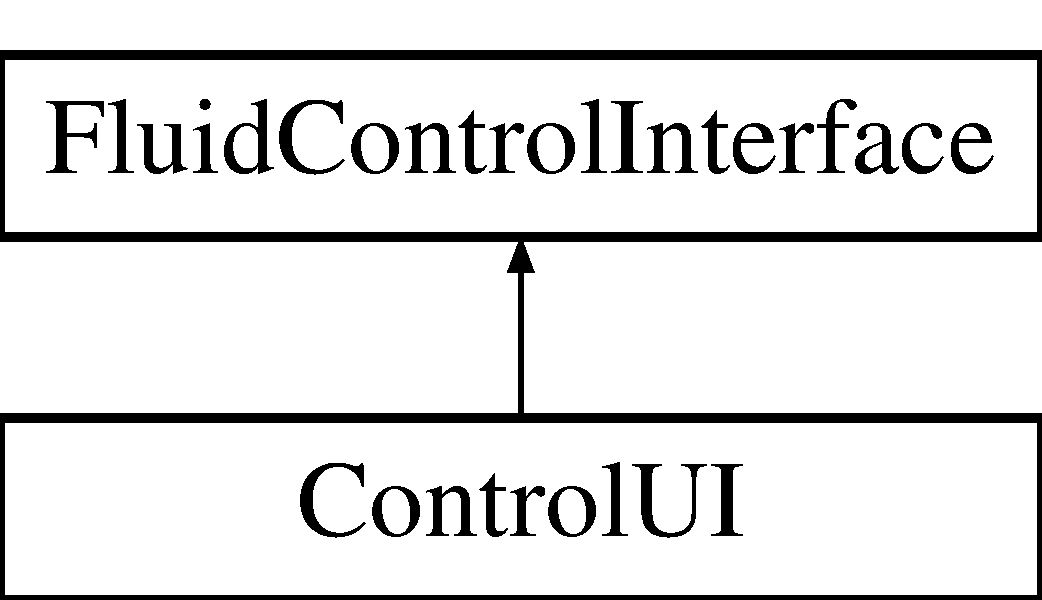
\includegraphics[height=2.000000cm]{class_fluid_control_interface}
\end{center}
\end{figure}
\subsection*{Public Member Functions}
\begin{DoxyCompactItemize}
\item 
\hyperlink{class_fluid_control_interface_a4cb172a43e95b2852f30807e9037a9d9}{Fluid\+Control\+Interface} ()
\end{DoxyCompactItemize}
\subsection*{Public Attributes}
\begin{DoxyCompactItemize}
\item 
Fl\+\_\+\+Double\+\_\+\+Window $\ast$ \hyperlink{class_fluid_control_interface_a94da1536108cd2bd24edefd8711ca510}{m\+Window}
\item 
Fl\+\_\+\+Box $\ast$ \hyperlink{class_fluid_control_interface_aad9032c096ff2feb1c72f534012282c9}{m\+Window\+Box}
\item 
Fl\+\_\+\+Button $\ast$ \hyperlink{class_fluid_control_interface_adc41c1528cbec12780e89140de2f8913}{m\+Btn\+Show\+Positions1}
\item 
Fl\+\_\+\+Button $\ast$ \hyperlink{class_fluid_control_interface_a3d74260a0b459e570427438dc5077db0}{m\+Btn\+Show\+Positions2}
\item 
Fl\+\_\+\+Button $\ast$ \hyperlink{class_fluid_control_interface_aedea42f561d246eb95442e13a88f8d23}{m\+Btn\+Show\+Positions3}
\item 
Fl\+\_\+\+Button $\ast$ \hyperlink{class_fluid_control_interface_a3827651fb223790ca880f23312266dde}{m\+Btn\+Show\+Positions4}
\item 
Fl\+\_\+\+Button $\ast$ \hyperlink{class_fluid_control_interface_a7d1930c1f10db9e39ce691f504b81387}{m\+Btn\+Start\+Loop}
\item 
Fl\+\_\+\+Button $\ast$ \hyperlink{class_fluid_control_interface_a885b36cf5c6e5ab82a2b6636579d840e}{m\+Btn\+Stop\+Loop}
\end{DoxyCompactItemize}


\subsection{Constructor \& Destructor Documentation}
\mbox{\Hypertarget{class_fluid_control_interface_a4cb172a43e95b2852f30807e9037a9d9}\label{class_fluid_control_interface_a4cb172a43e95b2852f30807e9037a9d9}} 
\index{Fluid\+Control\+Interface@{Fluid\+Control\+Interface}!Fluid\+Control\+Interface@{Fluid\+Control\+Interface}}
\index{Fluid\+Control\+Interface@{Fluid\+Control\+Interface}!Fluid\+Control\+Interface@{Fluid\+Control\+Interface}}
\subsubsection{\texorpdfstring{Fluid\+Control\+Interface()}{FluidControlInterface()}}
{\footnotesize\ttfamily Fluid\+Control\+Interface\+::\+Fluid\+Control\+Interface (\begin{DoxyParamCaption}{ }\end{DoxyParamCaption})}



\subsection{Member Data Documentation}
\mbox{\Hypertarget{class_fluid_control_interface_adc41c1528cbec12780e89140de2f8913}\label{class_fluid_control_interface_adc41c1528cbec12780e89140de2f8913}} 
\index{Fluid\+Control\+Interface@{Fluid\+Control\+Interface}!m\+Btn\+Show\+Positions1@{m\+Btn\+Show\+Positions1}}
\index{m\+Btn\+Show\+Positions1@{m\+Btn\+Show\+Positions1}!Fluid\+Control\+Interface@{Fluid\+Control\+Interface}}
\subsubsection{\texorpdfstring{m\+Btn\+Show\+Positions1}{mBtnShowPositions1}}
{\footnotesize\ttfamily Fl\+\_\+\+Button$\ast$ Fluid\+Control\+Interface\+::m\+Btn\+Show\+Positions1}

\mbox{\Hypertarget{class_fluid_control_interface_a3d74260a0b459e570427438dc5077db0}\label{class_fluid_control_interface_a3d74260a0b459e570427438dc5077db0}} 
\index{Fluid\+Control\+Interface@{Fluid\+Control\+Interface}!m\+Btn\+Show\+Positions2@{m\+Btn\+Show\+Positions2}}
\index{m\+Btn\+Show\+Positions2@{m\+Btn\+Show\+Positions2}!Fluid\+Control\+Interface@{Fluid\+Control\+Interface}}
\subsubsection{\texorpdfstring{m\+Btn\+Show\+Positions2}{mBtnShowPositions2}}
{\footnotesize\ttfamily Fl\+\_\+\+Button$\ast$ Fluid\+Control\+Interface\+::m\+Btn\+Show\+Positions2}

\mbox{\Hypertarget{class_fluid_control_interface_aedea42f561d246eb95442e13a88f8d23}\label{class_fluid_control_interface_aedea42f561d246eb95442e13a88f8d23}} 
\index{Fluid\+Control\+Interface@{Fluid\+Control\+Interface}!m\+Btn\+Show\+Positions3@{m\+Btn\+Show\+Positions3}}
\index{m\+Btn\+Show\+Positions3@{m\+Btn\+Show\+Positions3}!Fluid\+Control\+Interface@{Fluid\+Control\+Interface}}
\subsubsection{\texorpdfstring{m\+Btn\+Show\+Positions3}{mBtnShowPositions3}}
{\footnotesize\ttfamily Fl\+\_\+\+Button$\ast$ Fluid\+Control\+Interface\+::m\+Btn\+Show\+Positions3}

\mbox{\Hypertarget{class_fluid_control_interface_a3827651fb223790ca880f23312266dde}\label{class_fluid_control_interface_a3827651fb223790ca880f23312266dde}} 
\index{Fluid\+Control\+Interface@{Fluid\+Control\+Interface}!m\+Btn\+Show\+Positions4@{m\+Btn\+Show\+Positions4}}
\index{m\+Btn\+Show\+Positions4@{m\+Btn\+Show\+Positions4}!Fluid\+Control\+Interface@{Fluid\+Control\+Interface}}
\subsubsection{\texorpdfstring{m\+Btn\+Show\+Positions4}{mBtnShowPositions4}}
{\footnotesize\ttfamily Fl\+\_\+\+Button$\ast$ Fluid\+Control\+Interface\+::m\+Btn\+Show\+Positions4}

\mbox{\Hypertarget{class_fluid_control_interface_a7d1930c1f10db9e39ce691f504b81387}\label{class_fluid_control_interface_a7d1930c1f10db9e39ce691f504b81387}} 
\index{Fluid\+Control\+Interface@{Fluid\+Control\+Interface}!m\+Btn\+Start\+Loop@{m\+Btn\+Start\+Loop}}
\index{m\+Btn\+Start\+Loop@{m\+Btn\+Start\+Loop}!Fluid\+Control\+Interface@{Fluid\+Control\+Interface}}
\subsubsection{\texorpdfstring{m\+Btn\+Start\+Loop}{mBtnStartLoop}}
{\footnotesize\ttfamily Fl\+\_\+\+Button$\ast$ Fluid\+Control\+Interface\+::m\+Btn\+Start\+Loop}

\mbox{\Hypertarget{class_fluid_control_interface_a885b36cf5c6e5ab82a2b6636579d840e}\label{class_fluid_control_interface_a885b36cf5c6e5ab82a2b6636579d840e}} 
\index{Fluid\+Control\+Interface@{Fluid\+Control\+Interface}!m\+Btn\+Stop\+Loop@{m\+Btn\+Stop\+Loop}}
\index{m\+Btn\+Stop\+Loop@{m\+Btn\+Stop\+Loop}!Fluid\+Control\+Interface@{Fluid\+Control\+Interface}}
\subsubsection{\texorpdfstring{m\+Btn\+Stop\+Loop}{mBtnStopLoop}}
{\footnotesize\ttfamily Fl\+\_\+\+Button$\ast$ Fluid\+Control\+Interface\+::m\+Btn\+Stop\+Loop}

\mbox{\Hypertarget{class_fluid_control_interface_a94da1536108cd2bd24edefd8711ca510}\label{class_fluid_control_interface_a94da1536108cd2bd24edefd8711ca510}} 
\index{Fluid\+Control\+Interface@{Fluid\+Control\+Interface}!m\+Window@{m\+Window}}
\index{m\+Window@{m\+Window}!Fluid\+Control\+Interface@{Fluid\+Control\+Interface}}
\subsubsection{\texorpdfstring{m\+Window}{mWindow}}
{\footnotesize\ttfamily Fl\+\_\+\+Double\+\_\+\+Window$\ast$ Fluid\+Control\+Interface\+::m\+Window}

\mbox{\Hypertarget{class_fluid_control_interface_aad9032c096ff2feb1c72f534012282c9}\label{class_fluid_control_interface_aad9032c096ff2feb1c72f534012282c9}} 
\index{Fluid\+Control\+Interface@{Fluid\+Control\+Interface}!m\+Window\+Box@{m\+Window\+Box}}
\index{m\+Window\+Box@{m\+Window\+Box}!Fluid\+Control\+Interface@{Fluid\+Control\+Interface}}
\subsubsection{\texorpdfstring{m\+Window\+Box}{mWindowBox}}
{\footnotesize\ttfamily Fl\+\_\+\+Box$\ast$ Fluid\+Control\+Interface\+::m\+Window\+Box}



The documentation for this class was generated from the following files\+:\begin{DoxyCompactItemize}
\item 
src/\+F\+L\+U\+I\+D/\hyperlink{_fluid_control_interface_8h}{Fluid\+Control\+Interface.\+h}\item 
src/\+F\+L\+U\+I\+D/\hyperlink{_fluid_control_interface_8cxx}{Fluid\+Control\+Interface.\+cxx}\end{DoxyCompactItemize}

\hypertarget{class_fluid_price_control_u_i}{}\section{Fluid\+Price\+Control\+UI Class Reference}
\label{class_fluid_price_control_u_i}\index{Fluid\+Price\+Control\+UI@{Fluid\+Price\+Control\+UI}}


{\ttfamily \#include $<$Fluid\+Price\+Control.\+h$>$}

\subsection*{Public Member Functions}
\begin{DoxyCompactItemize}
\item 
\hyperlink{class_fluid_price_control_u_i_a2cda3cd2bdafd0550ffd992166db9f9b}{Fluid\+Price\+Control\+UI} ()
\end{DoxyCompactItemize}
\subsection*{Public Attributes}
\begin{DoxyCompactItemize}
\item 
Fl\+\_\+\+Double\+\_\+\+Window $\ast$ \hyperlink{class_fluid_price_control_u_i_a65c8356043b3a182a177cf4a52317124}{m\+\_\+window1}
\item 
Fl\+\_\+\+Button $\ast$ \hyperlink{class_fluid_price_control_u_i_a17dcc8d29c4170578c8305d0bbce0f89}{m\+\_\+btn\+Up}
\item 
Fl\+\_\+\+Button $\ast$ \hyperlink{class_fluid_price_control_u_i_a98213f3a52dd6c6b700f5a20f1cfa7ab}{m\+\_\+btn\+Down}
\item 
Fl\+\_\+\+Output $\ast$ \hyperlink{class_fluid_price_control_u_i_afcc19c4bc7bc7295854861d2f667f457}{m\+\_\+\+Bid\+Display}
\item 
Fl\+\_\+\+Output $\ast$ \hyperlink{class_fluid_price_control_u_i_a68a7585dc66f65459fa6c38c086299f8}{m\+\_\+\+Ask\+Display}
\item 
Fl\+\_\+\+Value\+\_\+\+Slider $\ast$ \hyperlink{class_fluid_price_control_u_i_ad57bb65dd4c67780a86158e5d2ac7b90}{m\+\_\+slider1}
\item 
Fl\+\_\+\+Button $\ast$ \hyperlink{class_fluid_price_control_u_i_a0f591e3a87e7a68d05d1b17625d7de87}{m\+\_\+btn\+Print}
\item 
Fl\+\_\+\+Button $\ast$ \hyperlink{class_fluid_price_control_u_i_a6a6870f04d6e93c70975e8dbc463c8eb}{m\+\_\+btn\+Live\+Data\+Console\+Print}
\item 
Fl\+\_\+\+Button $\ast$ \hyperlink{class_fluid_price_control_u_i_a298e80045e3c1ea8cabbc21b0b3138ca}{m\+\_\+btn\+Connect\+Live\+Data}
\item 
Fl\+\_\+\+Button $\ast$ \hyperlink{class_fluid_price_control_u_i_a41892b034300821670f3e585bdd191a3}{m\+\_\+btn\+Start\+Loop}
\item 
Fl\+\_\+\+Button $\ast$ \hyperlink{class_fluid_price_control_u_i_ad94515ca4f97533e76a67e04bf4411e4}{m\+\_\+btn\+Experiment}
\end{DoxyCompactItemize}


\subsection{Constructor \& Destructor Documentation}
\mbox{\Hypertarget{class_fluid_price_control_u_i_a2cda3cd2bdafd0550ffd992166db9f9b}\label{class_fluid_price_control_u_i_a2cda3cd2bdafd0550ffd992166db9f9b}} 
\index{Fluid\+Price\+Control\+UI@{Fluid\+Price\+Control\+UI}!Fluid\+Price\+Control\+UI@{Fluid\+Price\+Control\+UI}}
\index{Fluid\+Price\+Control\+UI@{Fluid\+Price\+Control\+UI}!Fluid\+Price\+Control\+UI@{Fluid\+Price\+Control\+UI}}
\subsubsection{\texorpdfstring{Fluid\+Price\+Control\+U\+I()}{FluidPriceControlUI()}}
{\footnotesize\ttfamily Fluid\+Price\+Control\+U\+I\+::\+Fluid\+Price\+Control\+UI (\begin{DoxyParamCaption}{ }\end{DoxyParamCaption})}



\subsection{Member Data Documentation}
\mbox{\Hypertarget{class_fluid_price_control_u_i_a68a7585dc66f65459fa6c38c086299f8}\label{class_fluid_price_control_u_i_a68a7585dc66f65459fa6c38c086299f8}} 
\index{Fluid\+Price\+Control\+UI@{Fluid\+Price\+Control\+UI}!m\+\_\+\+Ask\+Display@{m\+\_\+\+Ask\+Display}}
\index{m\+\_\+\+Ask\+Display@{m\+\_\+\+Ask\+Display}!Fluid\+Price\+Control\+UI@{Fluid\+Price\+Control\+UI}}
\subsubsection{\texorpdfstring{m\+\_\+\+Ask\+Display}{m\_AskDisplay}}
{\footnotesize\ttfamily Fl\+\_\+\+Output$\ast$ Fluid\+Price\+Control\+U\+I\+::m\+\_\+\+Ask\+Display}

\mbox{\Hypertarget{class_fluid_price_control_u_i_afcc19c4bc7bc7295854861d2f667f457}\label{class_fluid_price_control_u_i_afcc19c4bc7bc7295854861d2f667f457}} 
\index{Fluid\+Price\+Control\+UI@{Fluid\+Price\+Control\+UI}!m\+\_\+\+Bid\+Display@{m\+\_\+\+Bid\+Display}}
\index{m\+\_\+\+Bid\+Display@{m\+\_\+\+Bid\+Display}!Fluid\+Price\+Control\+UI@{Fluid\+Price\+Control\+UI}}
\subsubsection{\texorpdfstring{m\+\_\+\+Bid\+Display}{m\_BidDisplay}}
{\footnotesize\ttfamily Fl\+\_\+\+Output$\ast$ Fluid\+Price\+Control\+U\+I\+::m\+\_\+\+Bid\+Display}

\mbox{\Hypertarget{class_fluid_price_control_u_i_a298e80045e3c1ea8cabbc21b0b3138ca}\label{class_fluid_price_control_u_i_a298e80045e3c1ea8cabbc21b0b3138ca}} 
\index{Fluid\+Price\+Control\+UI@{Fluid\+Price\+Control\+UI}!m\+\_\+btn\+Connect\+Live\+Data@{m\+\_\+btn\+Connect\+Live\+Data}}
\index{m\+\_\+btn\+Connect\+Live\+Data@{m\+\_\+btn\+Connect\+Live\+Data}!Fluid\+Price\+Control\+UI@{Fluid\+Price\+Control\+UI}}
\subsubsection{\texorpdfstring{m\+\_\+btn\+Connect\+Live\+Data}{m\_btnConnectLiveData}}
{\footnotesize\ttfamily Fl\+\_\+\+Button$\ast$ Fluid\+Price\+Control\+U\+I\+::m\+\_\+btn\+Connect\+Live\+Data}

\mbox{\Hypertarget{class_fluid_price_control_u_i_a98213f3a52dd6c6b700f5a20f1cfa7ab}\label{class_fluid_price_control_u_i_a98213f3a52dd6c6b700f5a20f1cfa7ab}} 
\index{Fluid\+Price\+Control\+UI@{Fluid\+Price\+Control\+UI}!m\+\_\+btn\+Down@{m\+\_\+btn\+Down}}
\index{m\+\_\+btn\+Down@{m\+\_\+btn\+Down}!Fluid\+Price\+Control\+UI@{Fluid\+Price\+Control\+UI}}
\subsubsection{\texorpdfstring{m\+\_\+btn\+Down}{m\_btnDown}}
{\footnotesize\ttfamily Fl\+\_\+\+Button$\ast$ Fluid\+Price\+Control\+U\+I\+::m\+\_\+btn\+Down}

\mbox{\Hypertarget{class_fluid_price_control_u_i_ad94515ca4f97533e76a67e04bf4411e4}\label{class_fluid_price_control_u_i_ad94515ca4f97533e76a67e04bf4411e4}} 
\index{Fluid\+Price\+Control\+UI@{Fluid\+Price\+Control\+UI}!m\+\_\+btn\+Experiment@{m\+\_\+btn\+Experiment}}
\index{m\+\_\+btn\+Experiment@{m\+\_\+btn\+Experiment}!Fluid\+Price\+Control\+UI@{Fluid\+Price\+Control\+UI}}
\subsubsection{\texorpdfstring{m\+\_\+btn\+Experiment}{m\_btnExperiment}}
{\footnotesize\ttfamily Fl\+\_\+\+Button$\ast$ Fluid\+Price\+Control\+U\+I\+::m\+\_\+btn\+Experiment}

\mbox{\Hypertarget{class_fluid_price_control_u_i_a6a6870f04d6e93c70975e8dbc463c8eb}\label{class_fluid_price_control_u_i_a6a6870f04d6e93c70975e8dbc463c8eb}} 
\index{Fluid\+Price\+Control\+UI@{Fluid\+Price\+Control\+UI}!m\+\_\+btn\+Live\+Data\+Console\+Print@{m\+\_\+btn\+Live\+Data\+Console\+Print}}
\index{m\+\_\+btn\+Live\+Data\+Console\+Print@{m\+\_\+btn\+Live\+Data\+Console\+Print}!Fluid\+Price\+Control\+UI@{Fluid\+Price\+Control\+UI}}
\subsubsection{\texorpdfstring{m\+\_\+btn\+Live\+Data\+Console\+Print}{m\_btnLiveDataConsolePrint}}
{\footnotesize\ttfamily Fl\+\_\+\+Button$\ast$ Fluid\+Price\+Control\+U\+I\+::m\+\_\+btn\+Live\+Data\+Console\+Print}

\mbox{\Hypertarget{class_fluid_price_control_u_i_a0f591e3a87e7a68d05d1b17625d7de87}\label{class_fluid_price_control_u_i_a0f591e3a87e7a68d05d1b17625d7de87}} 
\index{Fluid\+Price\+Control\+UI@{Fluid\+Price\+Control\+UI}!m\+\_\+btn\+Print@{m\+\_\+btn\+Print}}
\index{m\+\_\+btn\+Print@{m\+\_\+btn\+Print}!Fluid\+Price\+Control\+UI@{Fluid\+Price\+Control\+UI}}
\subsubsection{\texorpdfstring{m\+\_\+btn\+Print}{m\_btnPrint}}
{\footnotesize\ttfamily Fl\+\_\+\+Button$\ast$ Fluid\+Price\+Control\+U\+I\+::m\+\_\+btn\+Print}

\mbox{\Hypertarget{class_fluid_price_control_u_i_a41892b034300821670f3e585bdd191a3}\label{class_fluid_price_control_u_i_a41892b034300821670f3e585bdd191a3}} 
\index{Fluid\+Price\+Control\+UI@{Fluid\+Price\+Control\+UI}!m\+\_\+btn\+Start\+Loop@{m\+\_\+btn\+Start\+Loop}}
\index{m\+\_\+btn\+Start\+Loop@{m\+\_\+btn\+Start\+Loop}!Fluid\+Price\+Control\+UI@{Fluid\+Price\+Control\+UI}}
\subsubsection{\texorpdfstring{m\+\_\+btn\+Start\+Loop}{m\_btnStartLoop}}
{\footnotesize\ttfamily Fl\+\_\+\+Button$\ast$ Fluid\+Price\+Control\+U\+I\+::m\+\_\+btn\+Start\+Loop}

\mbox{\Hypertarget{class_fluid_price_control_u_i_a17dcc8d29c4170578c8305d0bbce0f89}\label{class_fluid_price_control_u_i_a17dcc8d29c4170578c8305d0bbce0f89}} 
\index{Fluid\+Price\+Control\+UI@{Fluid\+Price\+Control\+UI}!m\+\_\+btn\+Up@{m\+\_\+btn\+Up}}
\index{m\+\_\+btn\+Up@{m\+\_\+btn\+Up}!Fluid\+Price\+Control\+UI@{Fluid\+Price\+Control\+UI}}
\subsubsection{\texorpdfstring{m\+\_\+btn\+Up}{m\_btnUp}}
{\footnotesize\ttfamily Fl\+\_\+\+Button$\ast$ Fluid\+Price\+Control\+U\+I\+::m\+\_\+btn\+Up}

\mbox{\Hypertarget{class_fluid_price_control_u_i_ad57bb65dd4c67780a86158e5d2ac7b90}\label{class_fluid_price_control_u_i_ad57bb65dd4c67780a86158e5d2ac7b90}} 
\index{Fluid\+Price\+Control\+UI@{Fluid\+Price\+Control\+UI}!m\+\_\+slider1@{m\+\_\+slider1}}
\index{m\+\_\+slider1@{m\+\_\+slider1}!Fluid\+Price\+Control\+UI@{Fluid\+Price\+Control\+UI}}
\subsubsection{\texorpdfstring{m\+\_\+slider1}{m\_slider1}}
{\footnotesize\ttfamily Fl\+\_\+\+Value\+\_\+\+Slider$\ast$ Fluid\+Price\+Control\+U\+I\+::m\+\_\+slider1}

\mbox{\Hypertarget{class_fluid_price_control_u_i_a65c8356043b3a182a177cf4a52317124}\label{class_fluid_price_control_u_i_a65c8356043b3a182a177cf4a52317124}} 
\index{Fluid\+Price\+Control\+UI@{Fluid\+Price\+Control\+UI}!m\+\_\+window1@{m\+\_\+window1}}
\index{m\+\_\+window1@{m\+\_\+window1}!Fluid\+Price\+Control\+UI@{Fluid\+Price\+Control\+UI}}
\subsubsection{\texorpdfstring{m\+\_\+window1}{m\_window1}}
{\footnotesize\ttfamily Fl\+\_\+\+Double\+\_\+\+Window$\ast$ Fluid\+Price\+Control\+U\+I\+::m\+\_\+window1}



The documentation for this class was generated from the following files\+:\begin{DoxyCompactItemize}
\item 
F\+L\+U\+I\+D/\hyperlink{_fluid_price_control_8h}{Fluid\+Price\+Control.\+h}\item 
F\+L\+U\+I\+D/\hyperlink{_fluid_price_control_8cxx}{Fluid\+Price\+Control.\+cxx}\end{DoxyCompactItemize}

\chapter{File Documentation}
\hypertarget{_fluid_control_interface_8cxx}{}\section{src/\+F\+L\+U\+I\+D/\+Fluid\+Control\+Interface.cxx File Reference}
\label{_fluid_control_interface_8cxx}\index{src/\+F\+L\+U\+I\+D/\+Fluid\+Control\+Interface.\+cxx@{src/\+F\+L\+U\+I\+D/\+Fluid\+Control\+Interface.\+cxx}}
{\ttfamily \#include \char`\"{}Fluid\+Control\+Interface.\+h\char`\"{}}\newline

\hypertarget{_fluid_control_interface_8h}{}\section{F\+L\+U\+I\+D/\+Fluid\+Control\+Interface.h File Reference}
\label{_fluid_control_interface_8h}\index{F\+L\+U\+I\+D/\+Fluid\+Control\+Interface.\+h@{F\+L\+U\+I\+D/\+Fluid\+Control\+Interface.\+h}}
{\ttfamily \#include $<$F\+L/\+Fl.\+H$>$}\newline
{\ttfamily \#include $<$F\+L/\+Fl\+\_\+\+Double\+\_\+\+Window.\+H$>$}\newline
{\ttfamily \#include $<$F\+L/\+Fl\+\_\+\+Button.\+H$>$}\newline
{\ttfamily \#include $<$F\+L/\+Fl\+\_\+\+Box.\+H$>$}\newline
\subsection*{Classes}
\begin{DoxyCompactItemize}
\item 
class \hyperlink{class_fluid_control_interface}{Fluid\+Control\+Interface}
\end{DoxyCompactItemize}

\hypertarget{_fluid_price_control_8cxx}{}\section{F\+L\+U\+I\+D/\+Fluid\+Price\+Control.cxx File Reference}
\label{_fluid_price_control_8cxx}\index{F\+L\+U\+I\+D/\+Fluid\+Price\+Control.\+cxx@{F\+L\+U\+I\+D/\+Fluid\+Price\+Control.\+cxx}}
{\ttfamily \#include \char`\"{}Fluid\+Price\+Control.\+h\char`\"{}}\newline

\hypertarget{_fluid_price_control_8h}{}\section{src/\+F\+L\+U\+I\+D/\+Fluid\+Price\+Control.h File Reference}
\label{_fluid_price_control_8h}\index{src/\+F\+L\+U\+I\+D/\+Fluid\+Price\+Control.\+h@{src/\+F\+L\+U\+I\+D/\+Fluid\+Price\+Control.\+h}}
{\ttfamily \#include $<$F\+L/\+Fl.\+H$>$}\newline
{\ttfamily \#include $<$F\+L/\+Fl\+\_\+\+Double\+\_\+\+Window.\+H$>$}\newline
{\ttfamily \#include $<$F\+L/\+Fl\+\_\+\+Button.\+H$>$}\newline
{\ttfamily \#include $<$F\+L/\+Fl\+\_\+\+Output.\+H$>$}\newline
{\ttfamily \#include $<$F\+L/\+Fl\+\_\+\+Value\+\_\+\+Slider.\+H$>$}\newline
\subsection*{Classes}
\begin{DoxyCompactItemize}
\item 
class \hyperlink{class_fluid_price_control_u_i}{Fluid\+Price\+Control\+UI}
\end{DoxyCompactItemize}

\hypertarget{_control_8cpp}{}\section{src/\+Control.cpp File Reference}
\label{_control_8cpp}\index{src/\+Control.\+cpp@{src/\+Control.\+cpp}}
{\ttfamily \#include \char`\"{}Control.\+h\char`\"{}}\newline
{\ttfamily \#include $<$iostream$>$}\newline
\subsection*{Namespaces}
\begin{DoxyCompactItemize}
\item 
 \hyperlink{namespace_mike}{Mike}
\end{DoxyCompactItemize}
\subsection*{Functions}
\begin{DoxyCompactItemize}
\item 
int \hyperlink{namespace_mike_ada7afe897748f668730c74456952e356}{Mike\+::frequency\+\_\+of\+\_\+primes} (int n)
\end{DoxyCompactItemize}

\hypertarget{_control_8h}{}\section{src/\+Control.h File Reference}
\label{_control_8h}\index{src/\+Control.\+h@{src/\+Control.\+h}}
{\ttfamily \#include \char`\"{}Fluid\+Price\+Control.\+h\char`\"{}}\newline
\subsection*{Classes}
\begin{DoxyCompactItemize}
\item 
class \hyperlink{class_mike_1_1_control}{Mike\+::\+Control}
\end{DoxyCompactItemize}
\subsection*{Namespaces}
\begin{DoxyCompactItemize}
\item 
 \hyperlink{namespace_mike}{Mike}
\end{DoxyCompactItemize}

\hypertarget{main_8cpp}{}\section{src/main.cpp File Reference}
\label{main_8cpp}\index{src/main.\+cpp@{src/main.\+cpp}}
{\ttfamily \#include $<$iostream$>$}\newline
{\ttfamily \#include \char`\"{}F\+L\textbackslash{}\+Fl.\+H\char`\"{}}\newline
{\ttfamily \#include \char`\"{}Control.\+h\char`\"{}}\newline
\subsection*{Namespaces}
\begin{DoxyCompactItemize}
\item 
 \hyperlink{namespace_mike}{Mike}
\end{DoxyCompactItemize}
\subsection*{Functions}
\begin{DoxyCompactItemize}
\item 
int \hyperlink{main_8cpp_ae66f6b31b5ad750f1fe042a706a4e3d4}{main} ()
\end{DoxyCompactItemize}


\subsection{Function Documentation}
\mbox{\Hypertarget{main_8cpp_ae66f6b31b5ad750f1fe042a706a4e3d4}\label{main_8cpp_ae66f6b31b5ad750f1fe042a706a4e3d4}} 
\index{main.\+cpp@{main.\+cpp}!main@{main}}
\index{main@{main}!main.\+cpp@{main.\+cpp}}
\subsubsection{\texorpdfstring{main()}{main()}}
{\footnotesize\ttfamily int main (\begin{DoxyParamCaption}{ }\end{DoxyParamCaption})}


%--- End generated contents ---

% Index
\backmatter
\newpage
\phantomsection
\clearemptydoublepage
\addcontentsline{toc}{chapter}{Index}
\printindex

\end{document}
